\subsection{Round 1 Solutions}\label{S::2023-S-1}

\begin{resources}
    Review by \resit{https://www.youtube.com/watch?v=Un1ZGsv8p2E}{Way Tan}
\end{resources}

\begin{question}[C]\label{Q::2023-S-1-1}
    Find the value of $m$ such that $2x^2 + 3x + m$ has a minimum value of 9.
    \begin{tasks}(5)
        \task $\dfrac98$
        \task $-\dfrac98$
        \task $\dfrac{81}8$
        \task $-\dfrac{81}{8}$
        \task $\dfrac{63}{8}$
    \end{tasks}
\end{question}
\begin{solution*}
    Completing the square, we obtain $2x^2 + 3x + m = 2(x + \frac34)^2 + (m - \frac98)$, whence the minimum value is $m - \frac98$. Hence, $m = 9 + \frac98 = \frac{81}{8}$.
\end{solution*}

\begin{question}[B]\label{Q::2023-S-1-2}
    Which of the following is true?
    \begin{tasks}(5)
        \task! $\sin{105\deg} - \cos{105}\deg = \dfrac{\sqrt3}{2}$
        \task! $\sin{105\deg} - \cos{105}\deg = \dfrac{\sqrt3}{\sqrt2}$
        \task! $\sin{105\deg} + \cos{105}\deg = \dfrac12$
        \task! $\sin{105\deg} + \cos{105}\deg = \dfrac1{\sqrt3}$
        \task! None of the above
    \end{tasks}
\end{question}
\begin{solution*}
    Observe that $105\deg = 60\deg + 45\deg$. Applying the sine and cosine angle addition formulae gives \[\sin{105\deg} = \frac{\sqrt3}{2}\bp{\frac12 + \frac{\sqrt3}{2}}, \quad \cos{105\deg} = \frac{\sqrt3}{2}\bp{\frac12 - \frac{\sqrt3}{2}}.\] Hence, $\sin{105\deg} - \cos{105}\deg = \frac{\sqrt2 \sqrt3}{2} = \frac{\sqrt3}{\sqrt2}$.
\end{solution*}

\clearpage
\begin{question}[B]\label{Q::2023-S-1-3}
    If $\log_{\sqrt2} x = 10 - 3\log_{\sqrt2} 10$, find $x$.
    \begin{tasks}(5)
        \task 0.32
        \task 0.032
        \task 0.0032
        \task 0.64
        \task 0.064
    \end{tasks}
\end{question}
\begin{solution*}
    Observe that the RHS can be rewritten as \[10 - 3\log_{\sqrt2} 10 = \log_{\sqrt2}\bp{\frac{{\sqrt2}^{10}}{10^3}} = \log_{\sqrt2} 0.032.\] Thus, $x = 0.032$.
\end{solution*}

\begin{question}[A]\label{Q::2023-S-1-4}
    If $(x-5)^2 + (y-5)^2 = 5^2$, find the smallest value of $(x+5)^2 + (y+5)^2$.
    \begin{tasks}(5)
        \task! $225 - 100\sqrt2$
        \task! $225 + 100\sqrt2$
        \task! $225\sqrt2$
        \task! $100\sqrt2$
        \task! None of the above
    \end{tasks}
\end{question}
\begin{solution*}
    Observe that this is equivalent to finding the square of the shortest distance between the circles with centres $(-5, -5)$ and $(5, 5)$, and radius 5. The shortest distance is attained along the line segment joining the centres of the two circles together. The shortest distance is thus \[\bp{\sqrt{(5+5)^2 + (5+5)^2} - 5}^2 = 225 - 100\sqrt2.\]
\end{solution*}

\begin{question}[C]\label{Q::2023-S-1-5}
    Suppose $\cos{180\deg + x} = \dfrac45$, where $90\deg < x < 180\deg$. Find $\tan{2x}$.
    \begin{tasks}(5)
        \task $\dfrac{24}{7}$
        \task $\dfrac{7}{24}$
        \task $-\dfrac{24}{7}$
        \task $-\dfrac{7}{24}$
        \task $-\dfrac{24}{25}$
    \end{tasks}
\end{question}
\begin{solution*}
    Note that $\cos{180\deg + x} = -\cos{x}$. Hence, $\cos{x} = -\frac45$, whence $\sin x = \sqrt{1 - (-\frac45)^2} = \frac35$ (note that $\sin x > 0$ since $x$ is in the second quadrant). Thus, \[\tan{2x} = \frac{\sin{2x}}{\cos{2x}} = \frac{2\sin x \cos x}{\cos^2 x - \sin^2 x} = -\frac{24}{7}.\]
\end{solution*}

\begin{question}[7]\label{Q::2023-S-1-6}
    Suppose the roots of $x^2 + 11x + 3 = 0$ are $p$ and $q$, and the roots of $x^2 + Bx - C = 0$ are $p+1$ and $q+1$. Find $C$.
\end{question}
\begin{solution}
    Let $f(x) = x^2 + 11x + 3$. Consider the map $M : x \mapsto x - 1$. Clearly, the roots of $Mf(x) = 0$ are $p+1$ and $q+1$. Hence, $x^2 + Bx - C = Mf(x)$. Since $-C$ is the $y$-intercept of $Mf(x) = 0$, we get $-C = Mf(0) = f(-1) = -7$. Thus, $C = 7$.
\end{solution}
\begin{solution}
    Note that $x^2 + 11x + 3 = (x-p)(x-q)$. By Vieta's formulas, we have $p + q = -11$. Hence,
    \begin{align*}
        x^2 + Bx - C &= (x-p - 1)(x-q - 1) = (x-p)(x-q) - (x-p) - (x-q) + 1 \\
        &= \bp{x^2 + 11x + 3} - \bp{2x + 11} + 1 = x^2 + 9x - 7,
    \end{align*}
    whence $C = 7$.
\end{solution}

\begin{question}[25]\label{Q::2023-S-1-7}
    If the smallest possible value of $(A-x)(23-x)(A+x)(23+x)$ is $-(48)^2$, find the value of $A$ if $A > 0$.
\end{question}
\begin{solution*}
    From the difference of squares identity, we clearly have \[(A-x)(23-x)(A+x)(23+x) = (x^2 - 23^2)(x^2 - A^2) = x^4 - (23^2 + A^2)x^2 + 23^2 A^2.\] Completing the square, we obtain \[\bp{x^2 - \frac{23^2 + A^2}{2}}^2 - \frac14 \bp{ 23^2 + A^2}^2.\] Thus, \[-(48)^2 = - \frac14 \bp{23^2 - A^2}^2,\] whence $A = 25$. Note that we reject $A = \sqrt{433}$ as we require $A$ to be an integer.
\end{solution*}

\begin{question}[3]\label{Q::2023-S-1-8}
    Find the smallest positive odd integer greater than 1 that is a factor of \[(2023)^{2023} + (2026)^{2026} + (2029)^{2029}.\]
\end{question}
\begin{solution*}
    Observe that $2023 \equiv 2026 \equiv 2029 \equiv 1 \pmod{3}$. Hence, \[(2023)^{2023} + (2026)^{2026} + (2029)^{2029} \equiv 0 \pmod{3},\] whence 3 is a factor of the above object.
\end{solution*}

\begin{question}[48]\label{Q::2023-S-1-9}
    Find the remainder of $7^{2023} + 9^{2023}$ when divided by 64.
\end{question}
\begin{solution*}
    Observe that $\varphi(64) = 32$. Since $2023 \equiv 7 \pmod{32}$, by Euler's theorem, one has \[7^{2023} + 9^{2023} \equiv 7^7 + 9^7 \equiv 7 \cdot 49^3 + 9 \cdot 81^3 \pmod{64}.\] Since $49 \equiv -15 = -(2^4 - 1) \pmod{64}$ and $81 \equiv 17 = (2^4 + 1) \pmod{64}$, we obtain \[7 \cdot 49^3 + 9 \cdot 81^3 \equiv 7(-15) + 9(17) \equiv 48 \pmod{64}.\]
\end{solution*}

\begin{question}[49]\label{Q::2023-S-1-10}
    Let $x, y, z > 1$ and let $A$ be a positive number such that $\log_x A = 30$, $\log_y A = 50$ and $\log_{xy}\bp{Az} = 150$. Find $(\log_A z)^2$.
\end{question}
\begin{solution*}
    Observe that $A = x^{30} = y^{50}$ and $Az = (xy)^{150}$. Hence, \[z = \frac{(xy)^{150}}{A} = \frac{\bp{A^{1/30} A^{1/50}}^{150}}{A} = A^7.\] Thus, $(\log_A z)^2 = 7^2 = 49$.
\end{solution*}

\begin{question}[1024]\label{Q::2023-S-1-11}
    Find the largest integer that is less than \[\frac{3^{10} - 2^{10}}{10!} \bp{\frac1{1! 9! 2} + \frac1{2! 8! 2^2} + \frac1{3! 7! 2^3} + \cdots + \frac1{9! 1! 2^9}}^{-1}.\] Here, $n! = n \cdot (n-1) \cdots 3 \cdot 2 \cdot 1$. For example, $5! = 5 \cdot 4 \cdot 3 \cdot 2 \cdot 1 = 120$.
\end{question}
\begin{solution*}
    Observe that \[\sum_{i = 1}^9 \frac{10!}{i! (10-i)!} \cdot \frac{1}{2^i} = \sum_{i = 1}^9 \binom{10}{i} \bp{\frac12}^i = \sum_{i = 0}^{10} \binom{10}{i} \bp{\frac12}^i - 2 = \bp{1 + \frac12}^{10} - 2,\] Hence,
    \begin{align*}
        &\frac{3^{10} - 2^{10}}{10!} \bp{\frac1{1! 9! 2} + \frac1{2! 8! 2^2} + \frac1{3! 7! 2^3} + \cdots + \frac1{9! 1! 2^9}}^{-1}\\
        &= \bp{3^{10} - 2^{10}} \bp{\sum_{i = 1}^9 \frac{10!}{i! (10-i)!} \cdot \frac{1}{2^i}}^{-1} = \bp{3^{10} - 2^{10}} \bs{\bp{\frac32}^{10} - 2}^{-1}\\
        &= 2^{10} \bp{1  + \frac{2^{10}}{3^{10} - 2^{10}}}.
    \end{align*}
    Clearly, $0 < \frac{2^{10}}{3^{10} - 2^{10}} < 1$. Thus, the largest integer less than the above object is $2^{10} = 1024$.
\end{solution*}

\begin{question}[84]\label{Q::2023-S-1-12}
    Consider the following simultaneous equations:
    \begin{align*}
        xy^2 + xyz &= 91\\
        xyz - y^2z &= 72
    \end{align*}
    where $x$, $y$, and $z$ are positive integers. Find the maximum value of $xz$.
\end{question}
\begin{solution*}
    Note that we have $xyz = 91 - xy^2 = 72 + y^2 z$, whence $19 = y^2 (x + z)$. By the AM-GM inequality, we have, \[\frac{19}{2y^2} = \frac{x + z}{2} \geq \sqrt{xz} \implies xz \leq \bp{\frac{19}{2y^2}}^2.\] To maximize $xz$, we must minimize $y$. Testing $y = 1$, we get \[\left\{\begin{aligned}
        x + xz = 91\\
        xz - z = 72
    \end{aligned}\right.\] Observe that $x + z = 19$, and $x$ is a factor of 91. Testing the only factors of 91 less than 19, which are 1, 7 and 13, we see that $x = 7$ and $z = 12$ is the only solution to the above system. Thus, $\max xz = 7 \cdot 12 = 84$.
\end{solution*}

\begin{question}[2]\label{Q::2023-S-1-13}
    Let $x$ be a real number such that \[\frac{\sin^4 x + \cos^4 x}{\sin^2 x + \cos^4 x} = \frac8{11}.\] Assuming $\sin^2 x > \dfrac12$, find the value of $\sqrt{28} \bp{\sin^4 x - \cos^4 x}$.
\end{question}
\begin{solution*}
    Cross-multiplying and writing $\cos^4 x = (1-\sin^2 x)^2$, we obtain a quadratic in $\sin^2 x$: \[14\sin^4 x - 14\sin^2 x + 3 = 0.\] Since $\sin^2 x > \frac12$, we have $\sin^2 x = \frac{7 + \sqrt{7}}{14}$. This immediately gives \[\sin^4 x = \frac{4 + \sqrt7}{14}, \quad \cos^4 x = \frac{4 - \sqrt7}{14}.\] Thus, \[\sqrt{28} \bp{\sin^4 x - \cos^4 x} = \sqrt{28} \cdot \frac{2\sqrt7}{14} = 2.\]
\end{solution*}

\begin{question}[160]\label{Q::2023-S-1-14}
    A sequence $a_1, a_2, \ldots$, is defined by \[a_1 = 5, \quad a_2 = 7, \quad a_{n+1} = \frac{a_n + 1}{a_{n-1}} \text{ for $n \geq 2$}.\] Find the value of $100 \times a_{2023}$.
\end{question}
\begin{solution*}
    Repeatedly applying the recurrence relation, we see that \[a_1 = 5, \quad a_2 =7, \quad a_3 = \frac85, \quad a_4 = \frac{13}{35}, \quad a_5 = \frac67, \quad a_6 = 5, \quad a_7 = 7.\] We thus see that the sequence has a period of 5. Since $2023 \equiv 3 \pmod{5}$, we have that $a_{2023} = a_3 = \frac85$, whence $100 \times a_{2023} = 160$.
\end{solution*}

\clearpage
\begin{question}[60]\label{Q::2023-S-1-15}
    Let $C$ be a constant such that the equation $5\cos x + 6 \sin x - C = 0$ have two distinct roots $a$ and $b$, where $0 < b < a < \pi$. Find the value of $61 \times \sin{a + b}$.
\end{question}
\begin{solution*}
    By the R-formula, one has $5\cos x + 6\sin x = \sqrt{61} \cos{x - \arctan \frac65}$. Note that $\frac\pi4 < \arctan{\frac65} < \frac\pi2$. Thus, if $C = \sqrt{61}\cos{\arctan \frac65}^+$, the equation $5\cos x + 6\sin x - C = 0$ will clearly have two solutions: namely $b = 0^+$ and $a = \bp{2\arctan \frac65}^-$. Hence, \[61 \sin{a + b} = 61\sin{2\arctan \frac65} = 61 \cdot 2 \sin{\arctan \frac65}\cos{\arctan\frac65} = 60 \]
\end{solution*}

\begin{question}[58]\label{Q::2023-S-1-16}
    In the diagram below, $CE$ is tangent to the circle at point $D$, $AD$ is the diameter of the circle, and $ABC$, $AFE$ are straight lines. It is given that $\frac{AB}{AC} = \frac{16}{41}$ and $\frac{AF}{AE} = \frac{49}{74}$. Let $\tan{\angle CAE} = \frac{m}{n}$, where $m$, $n$ are positive integers and $\frac{m}{n}$ is a fraction in its lowest form. Find the sum $m + n$.
    
    \begin{center}
        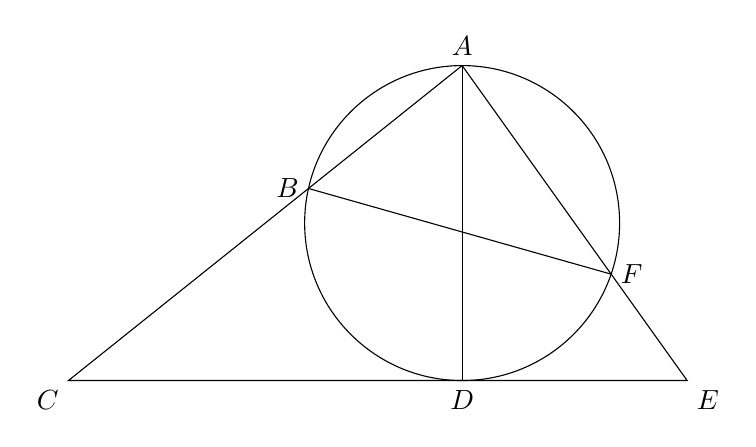
\begin{tikzpicture}[scale=2]
            \coordinate[label=above:$A$] (A) at (0, 1);
            \coordinate[label=left:$B$] (B) at (-40/41, 9/41);
            \coordinate[label=right:$F$] (F) at (35/37, -12/37);
            \coordinate[label=below:$D$] (D) at (0, -1);
            \coordinate[label=below right:$E$] (E) at (1.429, -1);
            \coordinate[label=below left:$C$] (C) at (-2.5, -1);

            \draw (0, 0) circle[radius=1];
            \draw (A) -- (E) -- (C) -- (A);
            \draw (A) -- (D);
            \draw (B) -- (F);
        \end{tikzpicture}
    \end{center}
\end{question}
\begin{center}
    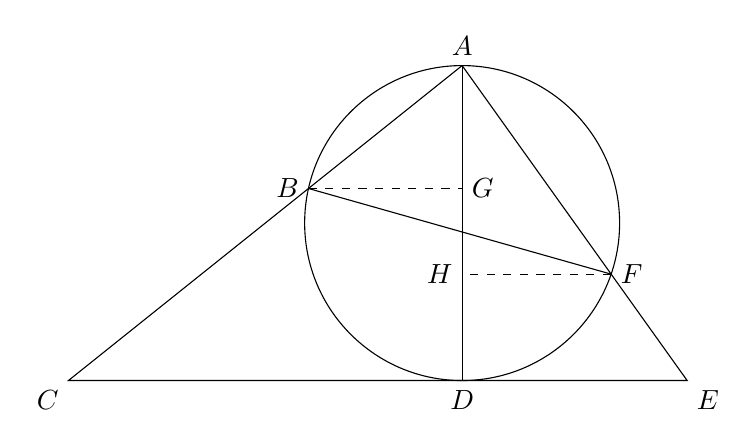
\begin{tikzpicture}[scale=2]
        \coordinate[label=above:$A$] (A) at (0, 1);
        \coordinate[label=left:$B$] (B) at (-40/41, 9/41);
        \coordinate[label=right:$F$] (F) at (35/37, -12/37);
        \coordinate[label=below:$D$] (D) at (0, -1);
        \coordinate[label=below right:$E$] (E) at (1.429, -1);
        \coordinate[label=below left:$C$] (C) at (-2.5, -1);
        \coordinate[label=right:$G$] (G) at (0, 9/41);
        \coordinate[label=left:$H$] (H) at (0, -12/37);

        \draw (0, 0) circle[radius=1];
        \draw (A) -- (E) -- (C) -- (A);
        \draw (A) -- (D);
        \draw (B) -- (F);
        \draw[dashed] (B) -- (G);
        \draw[dashed] (F) -- (H);
    \end{tikzpicture}
\end{center}
\begin{solution*}
    Let $(ABDF)$ be the unit circle. Then $AD = 2$. Let $G$ and $H$ be the foot of perpendiculars of $B$ and $F$ onto $AD$. By similar triangles, we have \[AG = \frac{16}{41} \cdot AD = \frac{32}{41}, \quad AH = \frac{49}{74} \cdot AD = \frac{49}{37}.\] Thus, $B$ has $y$-coordinate $1 - \frac{32}{41} = \frac{9}{41}$, while $F$ has $y$-coordinate $1 - \frac{49}{37} = -\frac{12}{37}$. Since $B$ and $F$ are on the unit circle, we have $\sin \a = \frac{9}{41}$ and $\sin \b = -\frac{12}{37}$, where $\a$ and $\b$ are the arguments of $B$ and $F$ respectively. Using the Pythagorean trigonometric identity, we obtain \[\cos \a = -\sqrt{1 - \bp{\frac{9}{41}}^2} = \frac{40}{41}, \quad \sin \b = \sqrt{1 - \bp{-\frac{12}{37}}^2} = \frac{35}{37},\] whence $B(-\frac{40}{41}, \frac{9}{41})$ and $F(\frac{35}{37}, -\frac{12}{37})$. Since $A(0, 1)$, we have \[\tan \angle ABG = \frac{BG}{AG} = \frac{40/41}{32/41} = \frac54, \quad \tan \angle FAH = \frac{FH}{AH} = \frac{35/37}{49/37} = \frac{5}{7}.\] Hence, \[\tan \angle CAE = \tan{\angle ABG + \angle FAH} = \frac{\tan \angle ABG + \tan \angle FAH}{1 - \tan \angle ABG \tan \angle FAH} = \frac{55}{3},\] whence $m + n = 55 + 3 = 58$.
\end{solution*}

\begin{question}[10]\label{Q::2023-S-1-17}
    In the diagram below, $AB$ is a diameter of the circle with centre $O$, $MN$ is a chord of the circle that intersects $AB$ at $P$, $\angle BON$ and $\angle MOA$ are acute angles, $\angle MPA = 45\deg$, $MP = \sqrt{56}$, and $NP = 12$. Find the radius of the circle.

    \begin{center}
        \begin{tikzpicture}[scale=0.6]
            \coordinate[label=above:$A$] (A) at (0, 5);
            \coordinate[label=below:$B$] (B) at (0, -5);
            \coordinate[label=above left:$M$] (M) at (-2.391, 4.391);
            \coordinate[label=below right:$N$] (N) at (4.391, -2.391);
            \coordinate[label=left:$O$] (O) at (0, 0);
            \coordinate[label=above right:$P$] (P) at (0, 2);
    
            \draw (O) circle[radius=5];
            \draw (M) -- (N);
            \draw (A) -- (B);
            
            \fill (P) circle[radius=2.5pt];
            \fill (O) circle[radius=2.5pt];
        \end{tikzpicture}
    \end{center}
\end{question}
\begin{solution*}
    Let $Q \in MN$ such that $OQ \perp MN$. Then $MQ = QN$, whence $PQ = 6 - \frac12 \sqrt{56} = 6 - \sqrt{14}$. Since $\angle OPQ = \angle MPA = 45\deg$ and $\angle PQO = 90\deg$, it follows that $\triangle OQP$ is a right-angled isosceles triangle, whence $OP = \sqrt{2} \bp{6 - \sqrt{14}}$. Using power of a point on $P$, we get \[\sqrt{56} \cdot 12 = \bp{r + OP}\bp{r - OP} = r^2 - OP^2 \implies r^2 = OP^2 + 24\sqrt{14} = 100.\] Thus, $r = 10$.
\end{solution*}

\clearpage
\begin{question}[1011]\label{Q::2023-S-1-18}
    Let $f(x) = \cos[2]{\frac{\pi x}{2}}$. Find the value of \[f\of{\frac1{2023}} + f\of{\frac2{2023}} + \cdots + f\of{\frac{2021}{2023}} + f\of{\frac{2022}{2023}}.\]
\end{question}
\begin{solution*}
    Observe that \[f(x) + f(1 - x) = \cos[2]{\frac{\pi x}{2}} + \cos[2]{\frac{\pi}2 - \frac{\pi x}{2}} = \cos[2]{\frac{\pi x}{2}} + \sin[2]{\frac{\pi x}{2}} = 1.\] Thus,
    \begin{align*}
        &f\of{\frac1{2023}} + f\of{\frac2{2023}} + \cdots + f\of{\frac{2021}{2023}} + f\of{\frac{2022}{2023}}\\
        &= \bs{f\of{\frac1{2023}} + f\of{\frac{2022}{2023}}} + \bs{f\of{\frac2{2023}} + f\of{\frac{2021}{2023}}} + \cdots + \bs{f\of{\frac{1011}{2023}} + f\of{\frac{1012}{2023}}}\\
        &= 1011.
    \end{align*}
\end{solution*}

\begin{question}[37]\label{Q::2023-S-1-19}
    Find the remainder when $3^{2023}$ is divided by 215.
\end{question}
\begin{solution*}
    Note that $215 = 5 \cdot 43$. Hence, $\varphi(215) = (5-1)(43-1) = 168$. Since $2023 \equiv 7 \pmod{168}$, by Euler's theorem, we have \[3^{2023} \equiv 3^7 \equiv 9 \cdot 243 \equiv 9 \cdot 28 \equiv 252 \equiv 37 \pmod{215}.\]
\end{solution*}

\begin{question}[514]\label{Q::2023-S-1-20}
    Find the sum of the prime divisors of 64000027.
\end{question}
\begin{solution*}
    Note that $64000027 = 20^6 + 3^3 = 400^3 + 3^3$. By the sum of cubes identity, we have \[64000027 = (400 + 3)(400^2 + 400 \cdot 3 + 3^2) = 403 \cdot 158809.\] Observe that $403 = 13 \cdot 31$, while $158809 = 7^3 \cdot 463$. Hence, the prime divisors of 64000027 are 7, 13, 31 and 463, whence their sum is 514.
\end{solution*}

\clearpage
\begin{question}[14161]\label{Q::2023-S-1-21}
    Let $\triangle ABC$ be an equilateral triangle. $D$, $E$, $F$ are points on the sides such that \[BD : DC = CE : EA = AF : FB = 2 : 1.\] Suppose the area of the triangle bounded by $AD$, $BE$ and $CF$ is 2023. Find the area of $\triangle ABC$.

    \begin{center}
        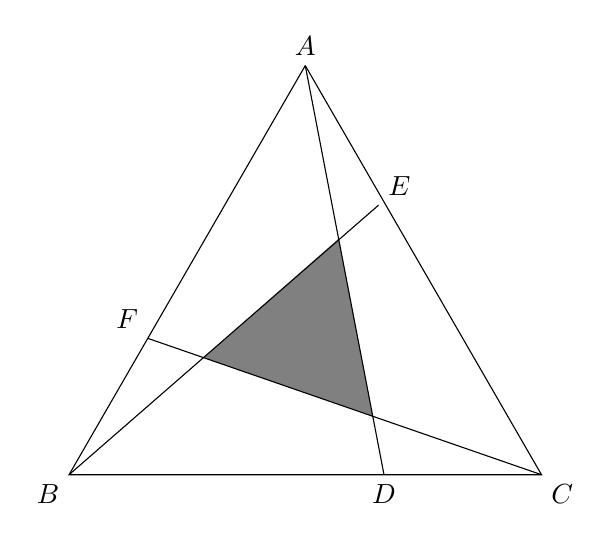
\begin{tikzpicture}[scale=2]
            \coordinate[label=above:$A$] (A) at (0, 2.598);
            \coordinate[label=below left:$B$] (B) at (-1.5, 0);
            \coordinate[label=below right:$C$] (C) at (1.5, 0);
            \coordinate[label=below:$D$] (D) at (0.5, 0);
            \coordinate[label=above right:$E$] (E) at (0.4656, 1.712);
            \coordinate[label=above left:$F$] (F) at (-1, 0.866);
            \coordinate (G) at (0.429, 0.371);
            \coordinate (H) at (0.213, 1.5);
            \coordinate (I) at (-0.646, 0.743);

            \fill[black!50] (G) -- (H) -- (I) -- (G);

            \draw (A) -- (B) -- (C) -- (A);
            \draw (A) -- (D);
            \draw (E) -- (B);
            \draw (C) -- (F);
        \end{tikzpicture}
    \end{center}
\end{question}
\begin{center}
    \begin{tikzpicture}[scale=2]
        \coordinate[label=above:$A$] (A) at (0, 2.598);
        \coordinate[label=below left:$B$] (B) at (-1.5, 0);
        \coordinate[label=below right:$C$] (C) at (1.5, 0);
        \coordinate[label=below:$D$] (D) at (0.5, 0);
        \coordinate[label=above right:$E$] (E) at (0.4656, 1.712);
        \coordinate[label=above left:$F$] (F) at (-1, 0.866);
        \coordinate[label=below left:$G$] (G) at (0.429, 0.371);
        \coordinate[label=below right:$H$] (H) at (0.213, 1.5);
        \coordinate[label=above:$I$] (I) at (-0.646, 0.743);

        \fill[black!50] (G) -- (H) -- (I) -- (G);

        \draw (A) -- (B) -- (C) -- (A);
        \draw (A) -- (D);
        \draw (E) -- (B);
        \draw (C) -- (F);

        \fill (G) circle[radius=1pt];
        \fill (H) circle[radius=1pt];
        \fill (I) circle[radius=1pt];

        \tkzMarkSegment[pos=.5,mark=|](G,H);
        \tkzMarkSegment[pos=.5,mark=|](I,H);
        \tkzMarkSegment[pos=.5,mark=|](G,I);

        \node[anchor=south east] at ($(A)!0.5!(F)$) {2};
        \node[anchor=south east] at ($(F)!0.5!(B)$) {1};
        \node[anchor=north] at ($(B)!0.5!(D)$) {2};
        \node[anchor=north] at ($(D)!0.5!(C)$) {1};
        \node[anchor=south west] at ($(C)!0.5!(E)$) {2};
        \node[anchor=south west] at ($(E)!0.5!(A)$) {1};
    \end{tikzpicture}
\end{center}
\begin{solution*}
    Let the side lengths of $\triangle ABC$ be 3 units. Let $G = CF \cap AD$, $H = AD \cap BE$ and $I = BE \cap CF$. By symmetry, $\triangle GHI$ is similar to $\triangle ABC$ and is hence also equilateral.
    
    Using Menalaus' theorem on $\triangle BEC$ and $\triangle ADC$, we get \[\frac{CA}{AE} \frac{EH}{HB} \frac{BD}{DC} = 1 \implies \frac{EH}{HB} = \frac16.\] Using Menalaus' theorem on $\triangle EIC$ and $\triangle AGC$, we have \[\frac{CA}{AE} \frac{EH}{HI} \frac{IG}{GC} = 1 \implies \frac{EH}{GC} = \frac13.\] Hence, $\frac{HI}{BE} = \frac37$. By the cosine rule, we obtain \[BE^2 = CE^2 + BC^2 - 2(CE)(BC)\cos \angle C \implies BE = \sqrt{7}.\] Thus, $HI = \frac3{\sqrt7}$, whence $\frac{AB}{HI} = \sqrt7$. Thus, \[[ABC] = \bp{\sqrt7}^2 [GHI] = 7 \cdot 2023 = 14161.\]
\end{solution*}

\begin{question}[47628]\label{Q::2023-S-1-22}
    Find the number of possible ways of arranging 10 ones and 11 zeros in a row such that there are in total 13 strings of ones and zeros. For example, \[1110001001110001\] consists of 4 strings of ones and 3 strings of zeros.
\end{question}
\begin{solution*}
    \case{1} Suppose the word starts with a 0. Then the thirteen strings must alternate as such: \[0101010101010,\] with seven strings of 0's and six strings of 1's. Since there are four 0's and four 1's left to place, by stars-and-bars, we have $\binom{4 + 7 - 1}{4} \binom{4 + 6 - 1}{4} = 26460$ unique combinations in this case.

    \case{2} Suppose the word starts with 1. Then the thirteen strings must alternate as such: \[1010101010101,\] with seven strings of 1's and six strings of 0's. Since there are three 1's and five 0's left to place, by stars-and-bars, we have $\binom{3 + 7 - 1}{3} \binom{5 + 6 - 1}{5} = 21168$ unique combinations in this case.

    Hence, there are a total oof $26460 + 21168 = 47628$ possible ways to arrange the 1's and 0's.
\end{solution*}

\begin{question}[66795]\label{Q::2023-S-1-23}
    Suppose there exist numbers $a$, $b$, $c$ and a function $f$ such that for any real numbers $x$ and $y$, \[f(x + y) + f(x - y) = 2f(x) + 2f(y) + ax + by + c.\] It is given that \[f(2) = 3, \quad f(3) = -5, \quad \text{ and } \quad f(5) = 7.\] Find the value of $f(123)$.
\end{question}
\begin{solution*}
    Let $P(x, y)$ be the assertion that $f(x + y) + f(x - y) = 2f(x) + 2f(y) + ax + by + c$.
    
    We first determine the values of $a$, $b$ and $c$. From $P(x, 0)$, we obtain \[f(x) + f(x) = 2f(x) + 2f(0) + ax + c \implies f(0) = -\frac{ax+c}{2}.\] Since $f(0)$ is a constant, it follows that $a = 0$, whence $f(0) = -\frac{c}{2}$. From $P(3, 2)$, we have \[f(5) + f(1) = 2f(3) + 2f(2) + 2b + c \implies f(1) = -11 + 2b + c. \tag{1}\] From $P(2, 1)$, we have \[f(3) + f(1) = 2f(2) + 2f(1) + b + c \implies f(1) = -11 - b - c. \tag{2}\] Equating (1) and (2) gives \[3b + 2c = 0. \tag{3}\] From $P(3, 1)$, we have \[f(4) + f(2) = 2f(3) + 2f(1) + b + c \implies f(4) = -35 - b - c.\] From $P(4, 1)$, we have \[f(5) + f(3) = 2f(4) + 2f(1) + b + c \implies 3b + 3c = -94. \tag{4}\] Solving (3) and (4) simultaneously gives $b = \frac{188}{3}$ and $c = -94$.

    Consider $P(x, 1)$. Then \[f(x+1) + f(x-1) = 2f(x) + 2f(1) + b + c \implies \bs{f(x+1) - f(x)} - \bs{f(x) - f(x-1)} = \frac{28}3.\] Let $a_n = f(n)$, where $n \in \NN$. We thus see that $a_n - a_{n-1}$ is in arithmetic progression with common difference $\frac{28}{3}$. Hence, \[a_n - a_{n-1} = (a_3 - a_2) + (n - 3)\frac{28}{3} \implies a_n = a_{n-1} + \frac{28}{3}n - 36.\] Thus, \[f(123) = a_{123} = a_2 + \sum_{k = 3}^{123} \bp{\frac{28}{3} k - 36} = 66795.\]
\end{solution*}

\begin{question}[454]\label{Q::2023-S-1-24}
    Let $f$ be a function such that for any non-zero number $x$, \[6xf(x) + 5x^2 f(1/x) + 10 = 0.\] Find the value of $f(10)$.
\end{question}
\begin{solution*}
    Plugging in $x = 10$ and $x = \frac1{10}$ into the functional equation, we get the following system of equations: \[\left\{\begin{aligned}
        60f(10) + 500f\of{\frac1{10}} + 10 = 0\\
        \frac6{10} f\of{\frac1{10}} + \frac5{100} f(10) + 10 = 0
    \end{aligned}\right.\] Solving, we obtain $f(10) = 454$.
\end{solution*}

\begin{question}[5]\label{Q::2023-S-1-25}
    Find the number of triangles such that all the sides are integers and the area equals the perimeter (in number).
\end{question}
\begin{solution*}
    Let the side lengths of the triangle be $a$, $b$ and $c$. Let $s = \frac{a + b + c}{2}$ be the semiperimeter of the triangle. From Heron's formula, we have \[a + b + c = \sqrt{s(s-a)(s-b)(s-c)},\] which gives \[16(a+b+c) = (-a+b+c)(a-b+c)(a+b-c).\] Let $x = -a + b + c$, $y = a-b+c$ and $z = a+b-c$. Then \[a = \frac{y+z}{2}, \quad b = \frac{z+x}{2}, \quad c = \frac{x+y}{2},\] whence \[16(x+y+z) = xyz.\] Clearly, $x$, $y$ and $z$ are all even. Substituting $x = 2X$, $y = 2Y$ and $z = 2Z$, we get \[4(X+Y+Z) = XYZ.\] Without loss of generality, suppose $X \leq Y \leq Z$. Then $XYZ \leq 12Z$, whence $XY \leq 12$. Additionally, $X^2 \leq XY \leq 12$, whence $X \leq 3$. We are thus left with the following few cases:

    \case{1} Suppose $X = 1$. Then \[4(1 + Y + Z) = YZ \implies (Y-4)(Z-4) = 20.\] This gives $(X, Y, Z) \in \bc{(1, 5, 24), (1, 6, 14), (1, 8, 9)}$.

    \case{2} Suppose $X = 2$. Then \[4(2 + Y + Z) = 2YZ \implies (Y-2)(Z-2) = 8.\] This gives $(X, Y, Z) \in \bc{(2, 3, 10), (2, 4, 6)}$.

    \case{3} Suppose $X = 3$. Then \[4(3 + Y + Z) = 3YZ \implies (3Y-4)(3Z-4) = 52.\] Note that $3Y - 4 \geq 3X - 4 = 8$. Since $52 = 1 \cdot 52 = 2 \cdot 26 = 4 \cdot 13$, there are no possibilities for $Y$. There are hence no solutions in this case.

    There are thus a total of 5 integer triangles whose perimeter is equal to its area in number.
\end{solution*}

